\chapter{Workload Metrics} \label{ch:workload}
The paper presented in chapter 2 was written before the workload concepts and modeling language semantics had settled into their current form.  Jared et al. \cite{FVHMS}, in concert with this work, published a paper in the FVHMS proceedings that expands on the concepts in chapter 2 but is also slightly outdated.  Thus we feel it expedient to summarize those aspects of the language which are critical to our metrics before we present the metrics themselves.  To assist in this effort we have prepared a simple scenario which includes a partial model and illustrations of the DiRG, DiTG, and labeled state transition system.

\section{Example Scenario}
In this scenario there are two people, Alice and Bob.  Alice is standing next to Bob listening to a friend on her cell phone.  Bob suddenly remembers that he wants to ask Alice out.  Not noticing that Alice is listening to her phone Bob starts to ask Alice on a date.  When this happens Alice looks at Bob and points to her phone, signaling to him that she is on the phone.  Bob stops talking and decides between waiting for her to finish or walking away.  Eventually Bob walks away.

\subsection{Actors}
From the scenario above we chose to create three Actors: A) Alice, B) Bob, and C) Cell Phone.  Actors represent any aspect of the system that has state.  An Actor can be anything, in our example we have two humans and a cell phone.  We could also create a sub-Actor which is part of a larger Actor, such as Bob's hair, and give it states like messy or combed.  Actors can also be very abstract or very detailed.  The more states an Actor contains, the more expressive it becomes.

\subsection{DiRG}
We express an Actor as a Directed Role Graph (DiRG).  A DiRG represents how an Actor is allowed to flow between states.  Figure~\ref{fig:ab_dirg} shows the DiRGs for both Alice and Bob as a state transition system.  We see that Alice is initially in a {\em Listening on phone} state while Bob is in the {\em Standing idle} state.  Alice can either stay in the {\em Listening on phone} state, shown by the looping transition, or move into the {\em Signaling Bob} state.  Once in the {\em Signaling Bob} state her only choice is to stay there forever or to return to the {\em Listening on phone} state.  Individually these DiRGs are of little value, together they begin to express the larger system.  We see from the labels on the DiRG that Alice and Bob are interacting with one another and influencing the transitions of the other.  Before we discuss Actor transitions we must first define the inter-Actor relationship that allows Actors to influence one another.

\begin{figure}[h]
\begin{center}
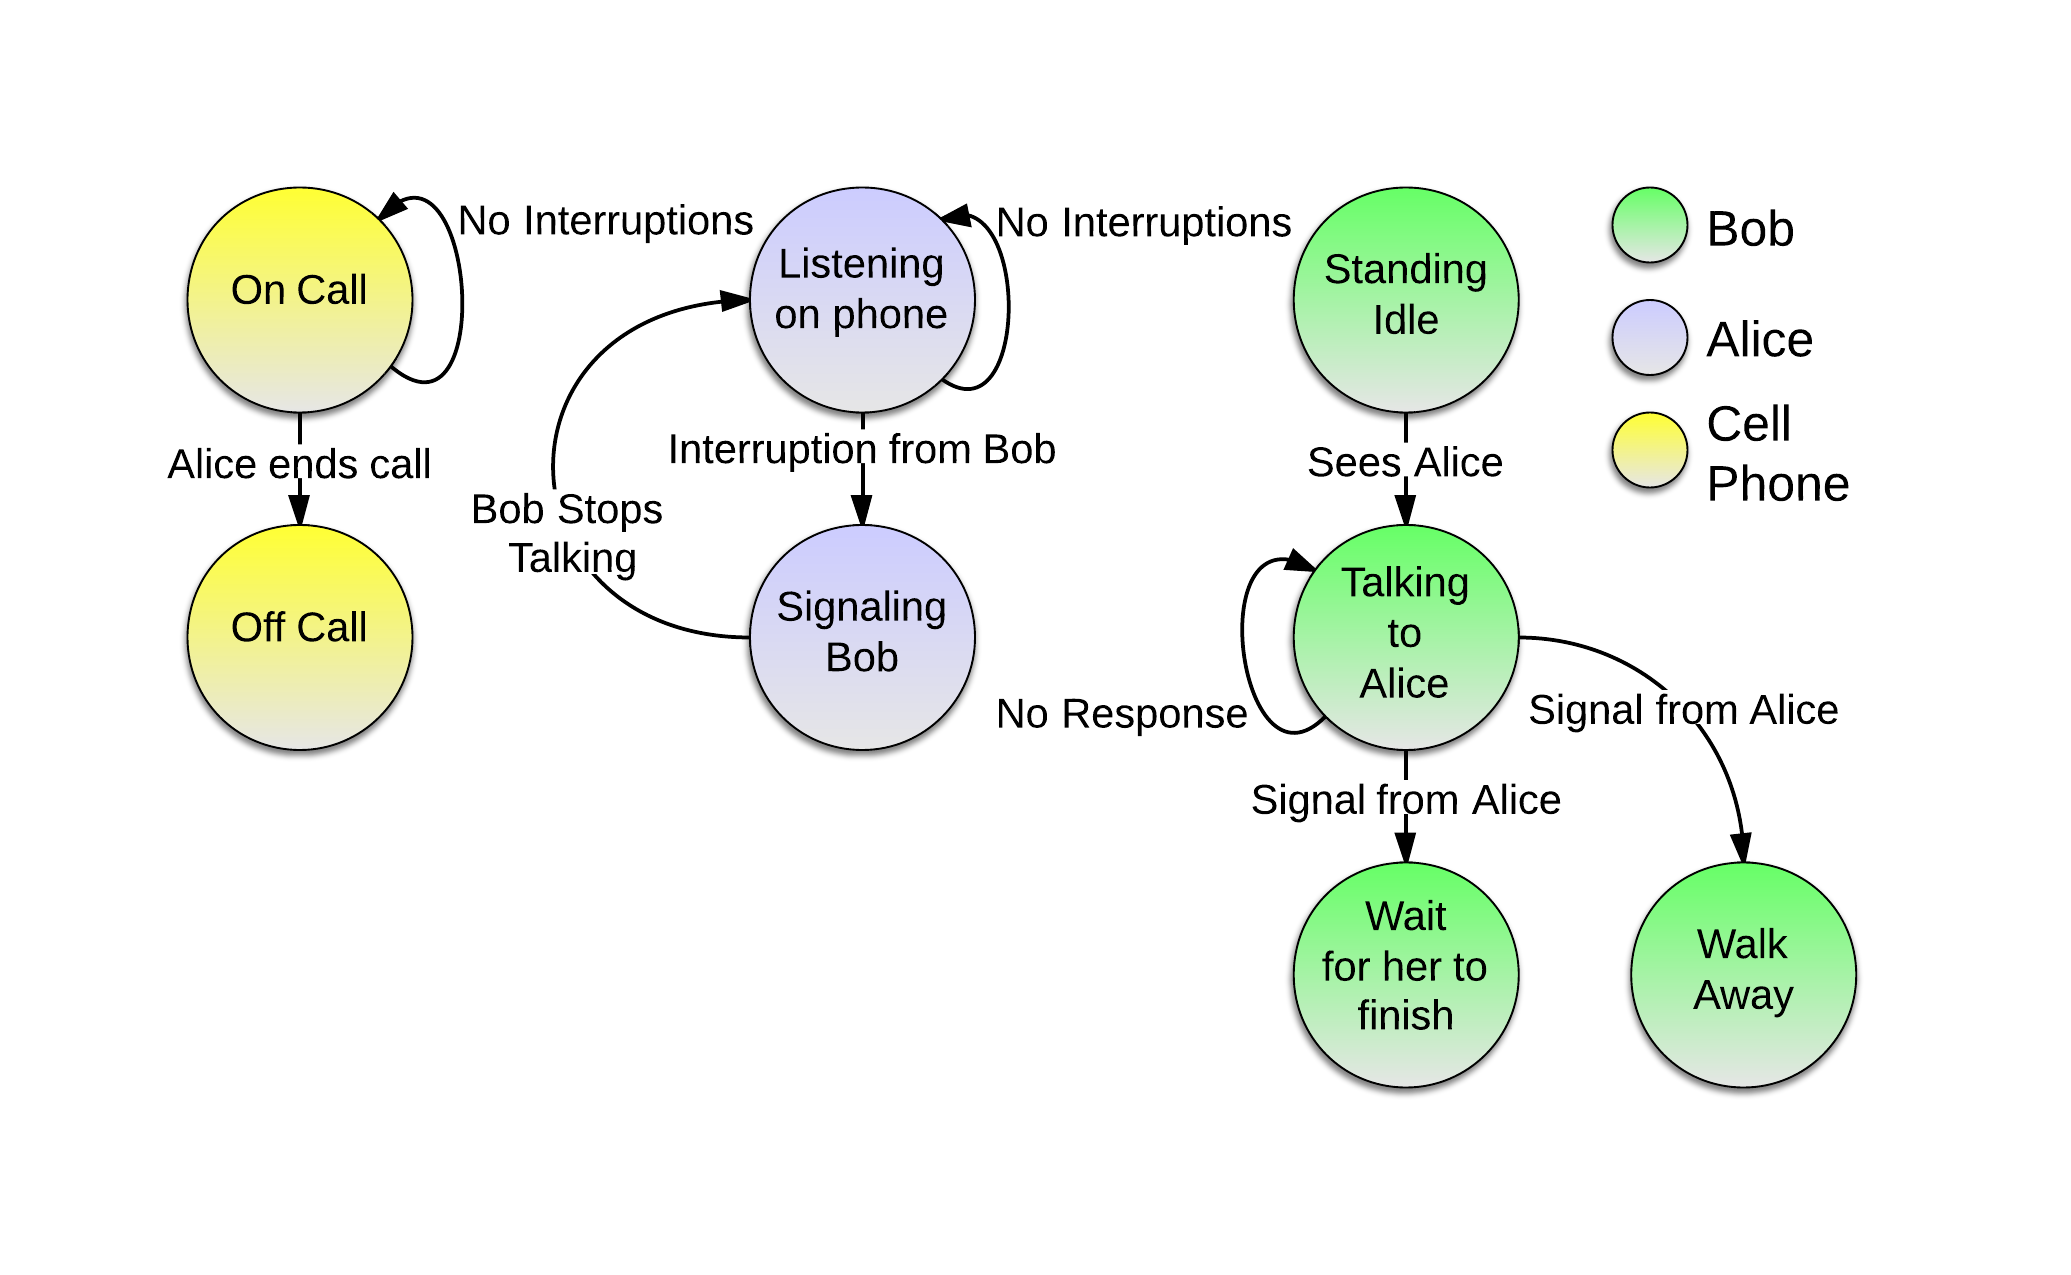
\includegraphics[width=\textwidth]{ab_dirg.png}
\caption{Directed Role Graph for Alice and Bob scenario}
\label{fig:ab_dirg}
\end{center}
\end{figure}

\subsection{Channels}
We define these inter-Actor connections as Channels.  A channel is a uni-directional communication medium which allows an Actor to send information to another Actor.  Each Channel is composed of a source Actor, a target Actor, and a type.  The source Actor sends information as {\em output}, the target Actor receives the information as {\em input}, and the type specifies which communication medium is being used.  In the case of Alice and Bob we use audio, visual, and manual Channels\cite{wickens2002multiple}, the case study in chapter \ref{ch:UASinNAS} also uses a Data channel that represents network communication.  

We also designate that each Channel can represent multiple layers of communication.  To show this we will use the visual channel from Alice to Bob as an example.  We can express Alice's {\em output}, Bob's {\em input}, as two different layers on the visual channel, one for Alice's body language, and another for her facial expressions.  This allows us to explicitly set how much data is being sent over the channel, it also allows us to express multiple visual inputs for Bob without creating a {\em channel conflict}.  A {\em channel conflict} occurs when an Actor is receiving input from two or more channels of the same type.  In our example scenario Alice is listening to her cell phone which uses an audio channel.  At the same time Bob is talking to Alice on a different audio channel.  Because Alice is receiving {\em input} on multiple audio channels she has an audio channel conflict.  

\subsection{DiTG}
To express a systems Channels we use a Directed Team Graph (DiTG)\cite{FVHMS}.  The DiTG defines all the channels that exist between the Actors within the system.  Figure \ref{fig:ab_ditg} shows the DiTG for our Alice and Bob scenario.  From the figure we can see that Alice has two channels to Bob, an audio and a visual and an audio channel to her cell phone.  We also see that Bob has two channels to Alice, an audio and a visual.  Lastly, the cell phone has an audio channel to Alice.  While the simplicity of this scenario makes it difficult to see the value of the DiTG, by combining the DiTG with the DiRG we have effectively constrained the Actor behavior and communication for the entire system.  With the constraints in place we are ready to define the behavior of the system, which we do with Transitions.

\begin{figure}[h]
\begin{center}
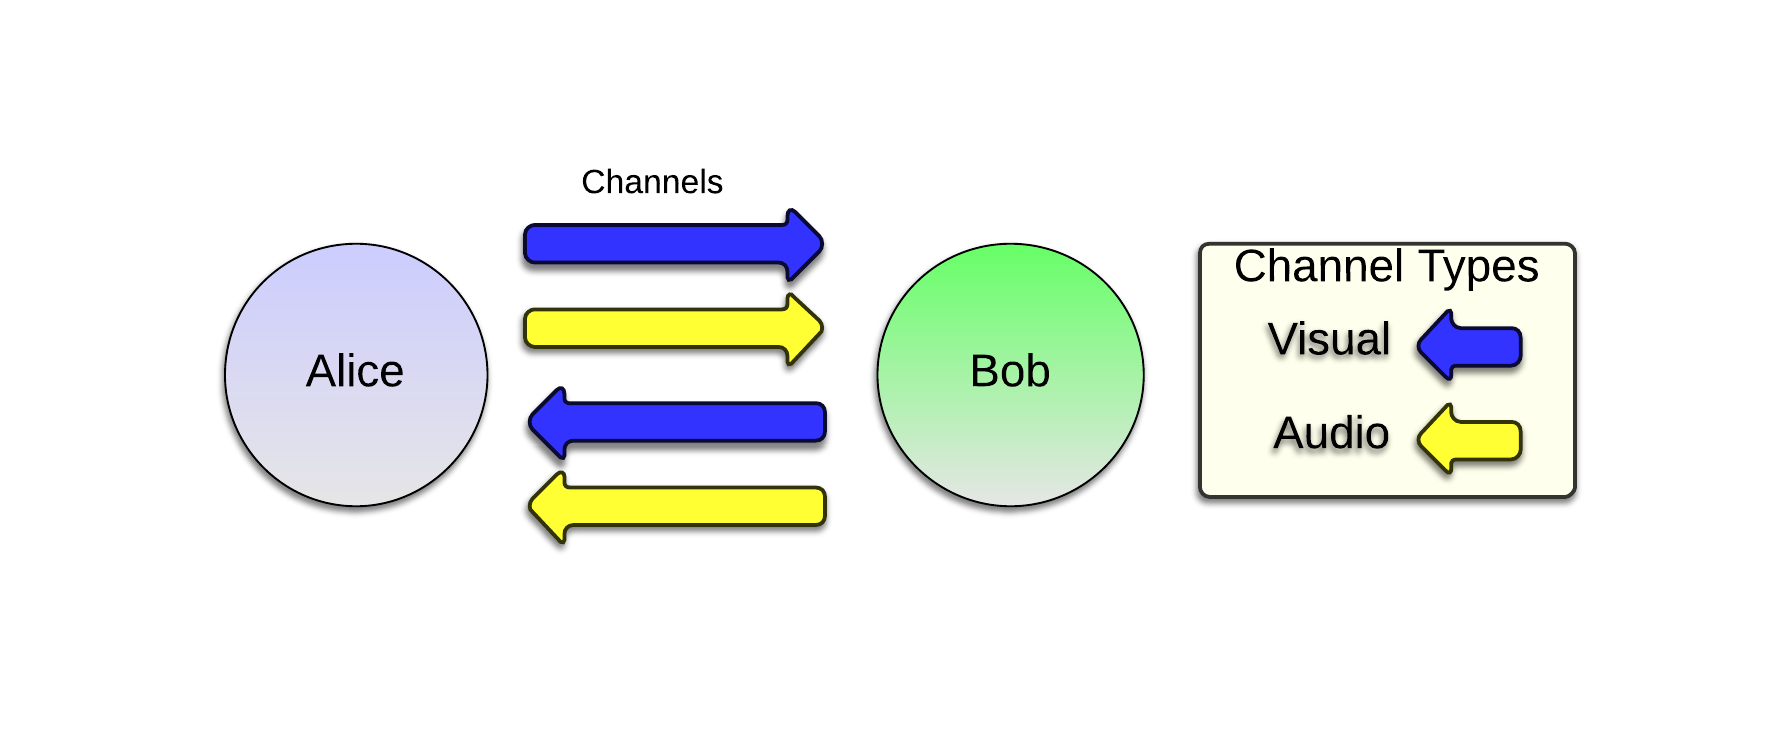
\includegraphics[width=\textwidth]{ab_ditg.png}
\caption{Directed Team Graph for Alice and Bob scenario}
\label{fig:ab_ditg}
\end{center}
\end{figure}

\subsection{Transitions}
Transitions represent an Actors behavior.  Transitions tells us about an Actors state, what caused the Actor to change state, and how that change effects the system.  Transitions are composed of a start state, an end state, a set of input equations, a set of outputs, a duration, and a priority.  The Transition start and end states are the states of the Actor and must not violate the DiRG.  

The Transition input equations are used to determine if the transition is enabled.  Each equation is composed of a source value, a predicate, and an expected value.  The source value is obtained from one of two sources, Channels or Memory.  Actor memory is an internal variable that allows an Actor to store and retrieve data.  For predicates we use equal to, less than, greater than, etc.  The structure of the input equations allows each equation to evaluate to a simple true or false.  If all input equations evaluate to true then the Transition is enabled.  

The Transition outputs contain all output generated by the transition as a set of target value pairs.  The target is the Channel or Memory variable that will receive the designated value.  The Transition duration is a range which represents the minimum and maximum number of time steps that a transition will remain {\em active} before it {\em fires}.  When an Actor decides to transition it selects an enabled transition to become {\em active}.  While a Transition is {\em active} the transition outputs are sent out but the Actor does not change state until the Transition {\em fires}.  We sometimes refer to inputs and outputs as being {\em active}, this implies that they are coming from an {\em active} Transition.  The final Transition element is priority.  Priority reflects how important a Transition is to the Actor relative to the other Transitions.  If multiple Transitions are enabled the Actor will choose the Transition with the highest priority.

\subsection{Labeled State Transition System}
The Model Abstraction Framework modeling language allows each of these concepts to be expressed in a model \ref{app:xmlparser}.  The model is then converted to a labeled state transition system that is sent to the simulator for metric collection.  We chose the labeled state transition system because the state transition system lends itself well to model checking while the label allows us to add specific data which relates to workload.  In our case the label translates directly to the transition input equations, outputs, duration, and priority.

\begin{figure}[h]
\begin{center}
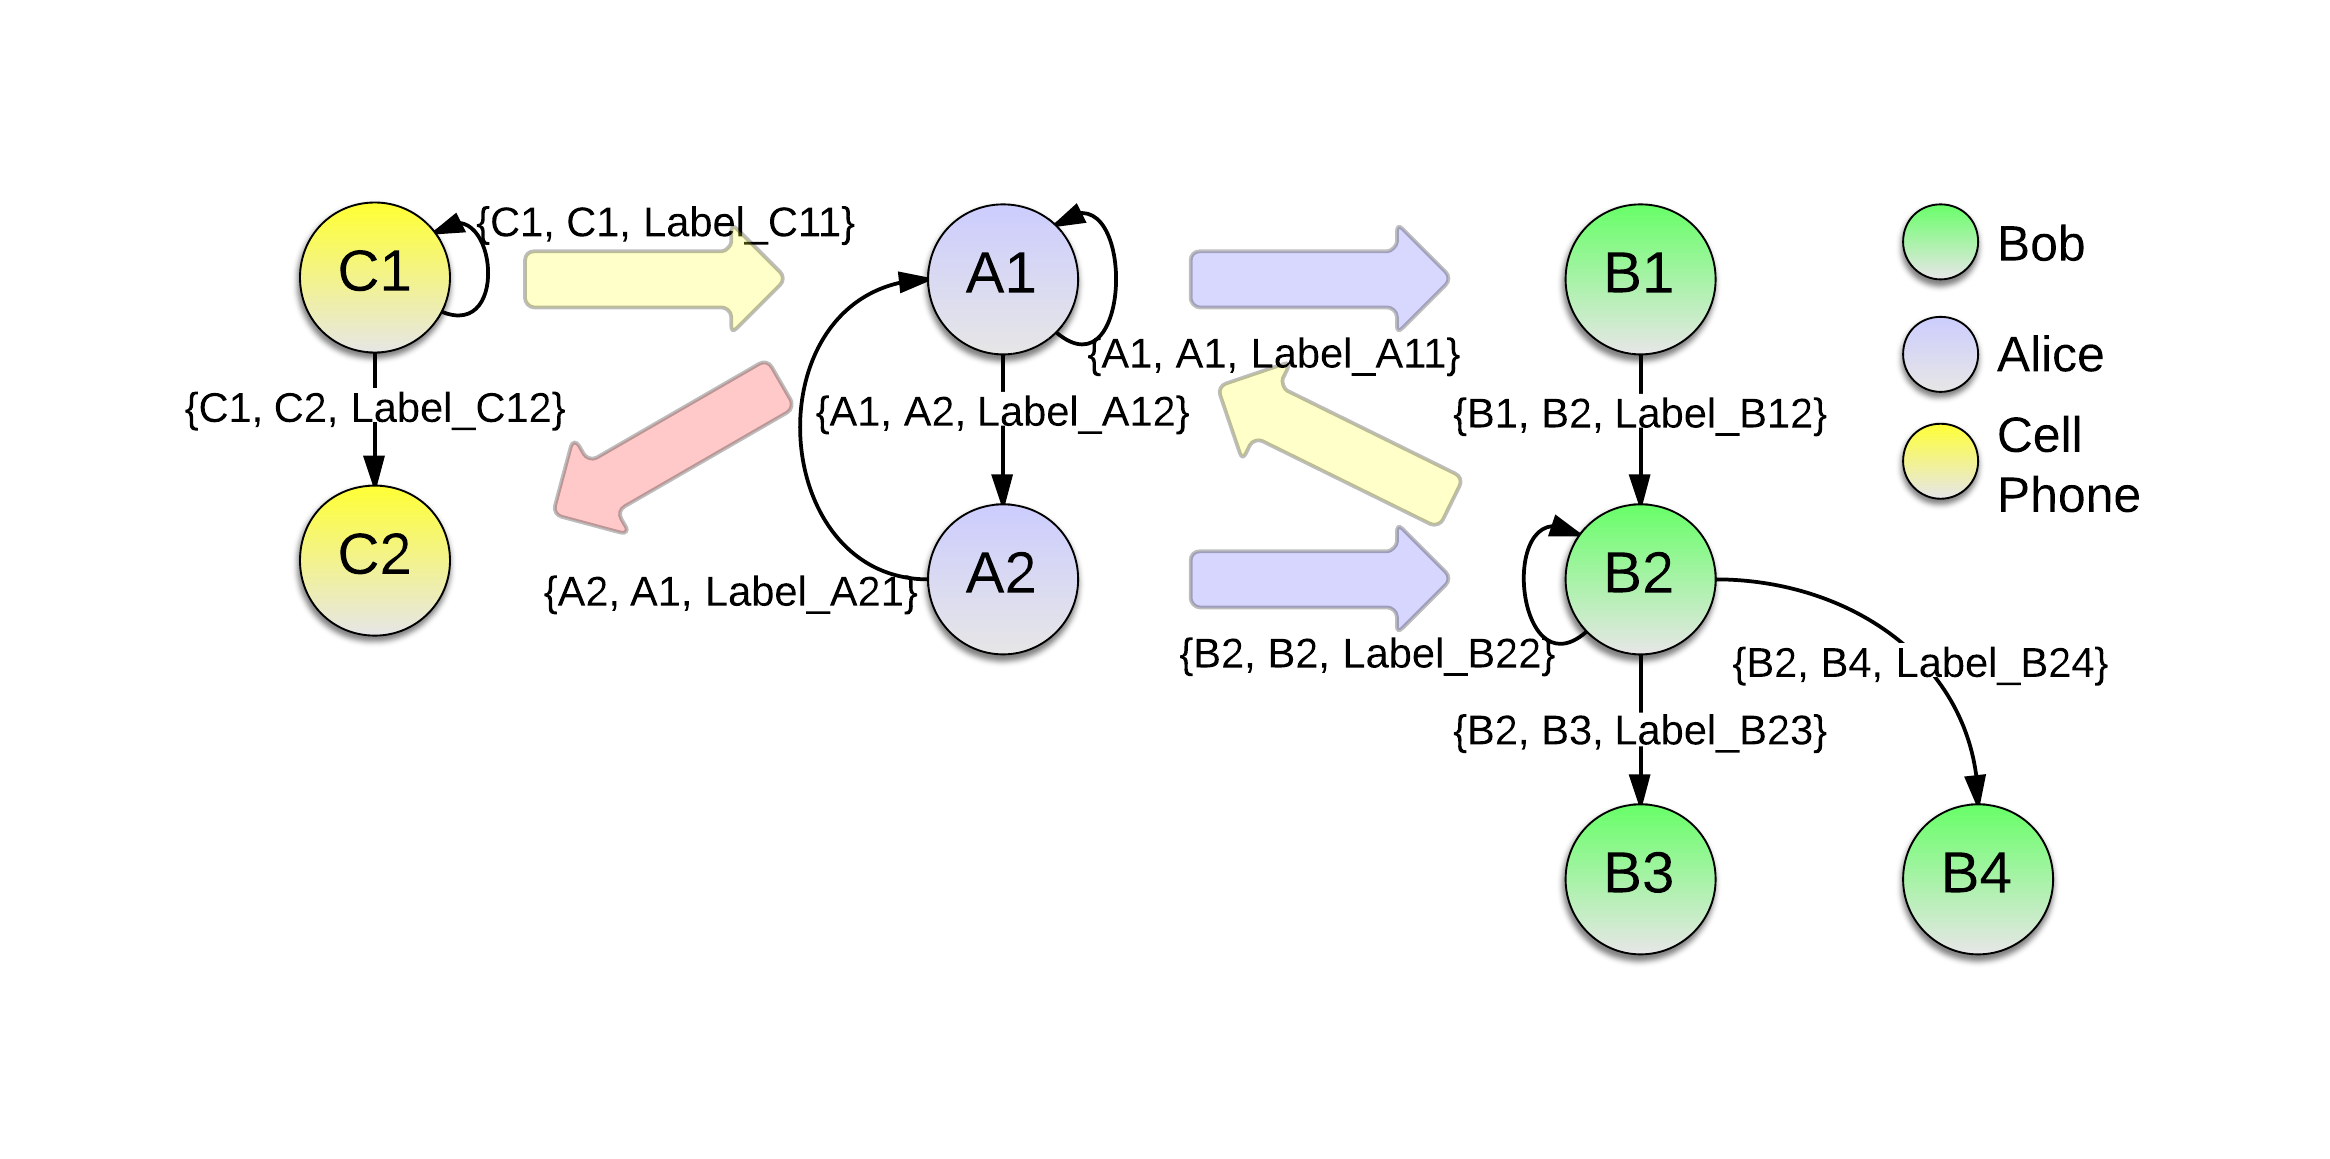
\includegraphics[width=\textwidth]{ab_lsts.png}
\caption{Labeled State Transition System for Alice and Bob scenario}
\label{fig:ab_lsts}
\end{center}
\end{figure}

In figure \ref{fig:ab_lsts} we can see that every transition has a label.  These labels are used by the simulator to determine if the transition is enabled, what channels will become {\em active}, and how long those channels should remain {\em active} before the state changes.  To make this clear we will describe $Label_A12$ of Alice's transition from the {\em Listening on phone} state to the {\em Signaling Bob} state.  From figure \ref{fig:ab_lsts} we see that when Bob is speaking to Alice there is an audio channel that is {\em active} (opaque yellow arrow).  The description on the transition implies that Bob's talking has somehow triggered the transition, to represent this in the label we create two input equations.  Audio channel from Bob does not equal null.  And audio channel from Cell Phone does not equal null.  This means that when Alice is listening to her cell phone if she hears Bob at the same time then this transition becomes enabled.  If she chooses to follow the transition then the transition becomes {\em active} and the transition outputs will become active.  In this case the output is a signal on the visual channel from Alice to Bob.  We will make the duration 5 seconds with a priority of 1.  

\subsection{Gathering Metrics}
Now that we have a basic understanding of the data that the simulator has access to during the simulation we can now discuss how we translate this data into meaningful metrics.  We will first discuss our baseline workload metric.  Afterwards we will describe the two workload metrics we created as part of this work.


\section{Adapted Wickens' Metric}
Since we are interested in metrics that reveal human workload we have chosen to replicate Wickens' computational model~\cite{wickens2002multiple}, shown in equations ~\ref{eq:resource_demand, eq:resource_conflict, eq:wickens_model}, using data gathered from the Model Abstraction Framework.  While this metric is a measure of resource demand and overlap, its close connection to human workload makes it an ideal baseline to compare against our own metrics.  

Wickens' computational model is based on the concept of tasks, where a task is some arbitrary unit of activity.  Wickens' model calculates the resource interference between two tasks through a resource demand component and a resource conflict component.  To keep the model simple and intuitive the resource demand for a single task was limited to 0-2, where 0 is an automated task and 2 is a difficult task.  Thus the total resource demand for two tasks ranges from 0 to 4.  See equation \ref{eq:resouce_demand}.

\begin{equation}
  R_{D}(T^{1}, T^{2}) = T_{demand}^{1} + T_{demand}^{2}
  \label{eq:resource_demand}
  \caption{Resource Demand}
\end{equation}

\begin{equation}
  R_{C}(T^{1}, T^{2}) = \sum_{dimension=1}^{4} \left\{
    \begin{array}{l l}
      1 & T_{dimension}^{1} = T_{dimension}^{2} \\
      0 & otherwise & \\
    \end{array}
  \label{eq:resource_conflict}
  \caption{Resource Conflict}
\end{equation}

For the resource conflict component two tasks are considered to have conflicting resources when they share resources within one of the dimensions illustrated in figure \ref{fig:multipleresourcetheory}.  The resource conflict value is the sum of the total number of dimensional conflicts between two tasks, as there are only four dimensions the resource conflict value will always be between 0 and 4.  See equation \ref{eq:resource_conflict}.  For example if $Task_{A}$ required a person to listen for distinct sounds while $Task_{B}$ required listening to a conversation the resource conflict would be 2.  One in the {\em Stages} dimension for perception, and another in the {\em Modalities} dimension for auditory.  Since one deals with spacial sound and the other verbal sound no resources are shared in the {\em Codes} dimension.  As neither task dealt with visual perception there are no conflicts in the {\em Visual Processing} dimension.

\begin{figure}[h]
\begin{center}
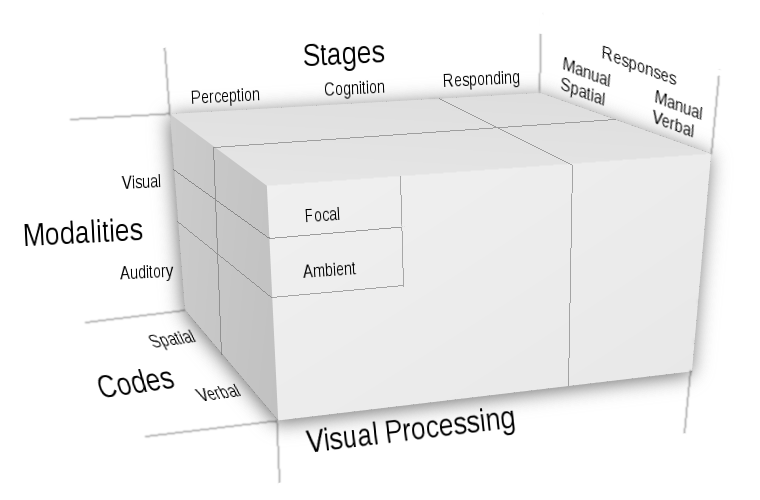
\includegraphics[width=6in]{multipleresourcetheory.png}
\caption{Multiple Resource Theory Dimensions~\cite{wickens2002multiple}}
\label{fig:multipleresourcetheory}
\end{center}
\end{figure}



\begin{equation}
  W(T_{1}, T_{2}) = R_{D}(T^{1}, T^{2}) + R_{C}(T^{1}, T^{2})
  \label{eq:wickens_model}
  \caption{Wickens' computational model}
\end{equation}



The difficulty with applying this model to our metrics is that we have removed the concept of tasks and replaced it with the notion of state and inputs.  The Model Abstraction Framework allows us to express tasks and other workload factors as resource, decision, and temporal elements by creating an actor state and modeling input consumption and output generation of that state.  This is beneficial for modeling vague or unknown systems since the modeler can focus on the input and output rather than specific task sets.  Unfortunately this focus on resource, decision, and temporal elements does not distinguish between tasks.  Any tasks are represented solely by an Actor's state, which may represent any number of tasks being performed, preventing a direct mapping from Wickens' model to our own. 


\subsection{Determining Task Difficulty}
In order to generate similar workload metrics as Wickens' model we needed a way to represent task difficulty (resource demand) in a similar fashion.  Using transition duration, the longer a task takes the more difficult it is, does not work because it prevents the modeler from placing an Actor into a long running simple task.  Inputs do not work since the data going over a channel do not always reflect resource demand, shown by a human's ability to tune out certain inputs.  Further examination revealed that we had no way to explicitly define an Actor's resource demand with the Model Abstraction Framework.  Wickens' model allows the modeler to subjectively set the task difficulty from their own experience and intuition.  While it is possible to implicitly define task difficulty from resource, decision, and temporal elements of the model we believe that Wickens' approach, allowing the modeler to subjectively define this value, will be more accurate.  To accomodate this we chose to add this subjective difficulty value to the Model Abstraction Framework under the label of Actor Load.


  
\subsection{Actor Load}
Actor Load represents an abstraction of the load an Actor is under while in a specific state.  Similar to Wickens' model, we have abstracted the Actor Load into an integer value ranging from 0-4.  An Actor Load of 0 represents little to no load on the actor.  These are automated or transitional states where the Actor is idle or has minimal contact with the system.  An Actor Load of 4 represents simultaneously performing multiple high difficulty tasks.  These are states where an Actor is pushed to the limit of their cognitive capabilities. Any value between 0 and 4 is some combination of task difficulty and the number of tasks being performed.  Actor Load is subjectively assigned to an Actors' state by the modeler.

\subsection{Determining Dimensional Conflicts}
To calculate the dimensionality of resource conflicts we need a way to determine when multiple tasks are being performed.  Since the Model Abstraction Framework does not define specific tasks we must find another method to approximate when multiple tasks are being performed.  We accomplish this by making the assumption that if an Actor has input from multiple sources then multiple tasks are being performed.



With this assumption we are ready to calculate dimensional conflicts as illustrated in Figure~\ref{fig:multipleresourcetheory}.
For the Stage dimension (perception, cognition, response) we check to see if there are multiple sources of input or multiple targets for output.  If there are then we increment the dimensionality as shown in equation~\ref{eq:stage_dimension}.  

For the Modality dimension (Audio, Visual) we check if there is more than a single active channel, input or output, of type audio or visual.  If there is then we increment the dimensionality as shown in equation~\ref{eq:modality_dimension}.

For the Focus dimension we check if there is more than one target for manual outputs, if there are then we increment the dimensionality as shown in equation~\ref{eq:focus_dimension}.  We do not check inputs as we have no way of distinguishing if a visual channel has focus.  This may need to be addressed in future work. 

For the Codes dimension (Spatial, Verbal) we check that the total number of audio inputs and outputs is greater than 1 or that the total number of visual inputs, visual outputs, and manual outputs is greater than 1.  If either value is greater than 1 then we increment the dimensionality as shown in equation~\ref{eq:codes_dimension}.


\begin{equation}
D_{S}(Inputs, Outputs) = \left\{ 
  \begin{array}{l l}
    1, Inputs_{Sources} > 1 & \quad \text{Multiple Input Sources}\\
    1, Outputs_{Targets} > 1 & \quad \text{Multiple Output Targets}\\
    0, otherwise
  \end{array}
  \right.
  \label{eq:stage_dimension}
\end{equation}

\begin{equation}
D_{M}(Inputs, Outputs) = \left\{ 
  \begin{array}{l l}
    1, Inputs_{Active}^{Audio/Visual} > 1 & \quad \text{Multiple Active Inputs}\\
    1, Outputs_{Active}^{Audio/Visual} > 1 & \quad \text{Multiple Active Outputs}\\
    0, otherwise
  \end{array}
  \right.
  \label{eq:modality_dimension}
\end{equation}

\begin{equation}
D_{F}(Outputs) = \left\{ 
  \begin{array}{l l}
    1, Outputs_{Target}^{Manual} > 1 & \quad \text{Multiple Manual Output Targets}\\
    0, otherwise
  \end{array}
  \right.
  \label{eq:focus_dimension}
\end{equation}

\begin{equation}
D_{C}(Inputs, Outputs) = \left\{ 
  \begin{array}{l l}
    1, Inputs^{Audio} + Outputs^{Audio} > 1\\
    1, Inputs^{Visual/Manual} + Outputs^{Visual/Manual} > 1\\
    0, otherwise
  \end{array}
  \right.
  \label{eq:codes_dimension}
\end{equation}


\subsection{Adapted Wickens' Model}
Using the adaptations mentioned in this section we are able to replicate Wickens' model within the Model Abstraction Framework by summing the Actor Load with the dimensional conflict values.  Equation~\ref{eq:adapted_wickens_model}.  As the model values are calculated differently than Wickens' model we will refer to this model as an adapted Wickens' model.  We propose to use this adapted Wickens' model as a baseline comparison for our metrics since the core elements of the adapted Wickens' model are fundamentally the same as those in the original.  

\begin{equation}
W(ActorLoad, D_{S}, D_{M}, D_{F}, D_{C}) = \left\{ 
  \begin{array}{l l}
    ActorLoad \in \{0,1,2,3,4\}\\
    ActorLoad + D_{S} + D_{M} + D_{F} + D_{C}
  \end{array}
  \right.
  \label{eq:adapted_wickens_model}
\end{equation}

\section{Resource Workload}
Describe what it is, point reader towards FVHMS paper.  Present the metric itself with the equation.
Intuition behind it?

\section{Decision Workload}
Describe what decision workload is, point reader towards FVHMS paper.  Present the metric itself with the equation.
Intuition behind it?

